\usetikzlibrary{fit,matrix}
\usetikzlibrary{arrows.meta,calc,shapes}
\providecommand{\computer}{%
    
\includegraphics[width=0.7cm]{../common/Noun_project_216.pdf}
}
\providecommand{\computerAlt}{%
    
\includegraphics[width=0.8cm]{../common/Noun_project_alt_cpu.pdf}
}
\providecommand{\switch}{%
    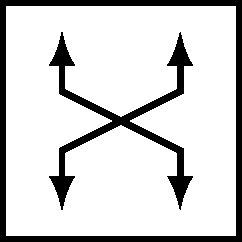
\includegraphics[width=0.8cm]{../common/fig-switch.pdf}
}
\providecommand{\router}{%
    
\includegraphics[width=0.8cm]{../common/fig-router.pdf}
}

\begin{frame}[fragile]{networks v routers (LS)}
\tikzset{
    mynode/.style={draw,circle,very thick,font=\small},
    myedge/.style={draw,ultra thick},
    computer/.style={inner sep=0mm,outer sep=0mm,execute at begin node={\computer}},
    switch/.style={inner sep=0mm,outer sep=0mm,execute at begin node={\switch}},
    router/.style={inner sep=0mm,outer sep=0mm,execute at begin node={\router}},
    port/.style={pos=0.95,fill=white,circle,draw,inner sep=0mm},
    port beginning/.style={pos=0.05,fill=white,circle,draw,inner sep=0mm},
    connect/.style={draw,thick,Latex-Latex},
    msg link/.style={draw,violet,line width=1.2mm,-Latex},
    msg data/.style={draw=violet,line width=0.8mm,fill=white,align=left,font=\fontsize{9}{10}\selectfont,align=left},
}
\begin{tikzpicture}
\foreach \x/\offX/\offY in {1/0/0,2/3/0} {
    \begin{scope}[xshift=\offX cm,yshift=\offY cm]
    \node[computer] (c\x-a) at (0, 0) {};
    \node[computer] (c\x-b) at (1, 0) {};
    \node[switch] (s\x) at (0.5, -1) {};
    \draw[connect] (c\x-a) -- (s\x);
    \draw[connect] (c\x-b) -- (s\x);
    \end{scope}
}
\foreach \x/\offX/\offY in {3/0/-6} {
    \begin{scope}[xshift=\offX cm,yshift=\offY cm]
    \node[computer] (c\x-a) at (0, 0) {};
    \node[computer] (c\x-b) at (1, -.5) {};
    \node[computer] (c\x-c) at (2, -.5) {};
    \node[switch] (s\x) at (0.5, 2) {};
    \node[switch] (s\x-b) at (1.5, 1) {};
    \draw[connect] (c\x-a) -- (s\x);
    \draw[connect] (c\x-b) -- (s\x-b);
    \draw[connect] (c\x-c) -- (s\x-b);
    \draw[connect] (s\x) -- (s\x-b);
    \end{scope}
}
\node[switch] (s4) at (4, -5) {};
\node[router,label={south:R1}] (r1) at (-1, -3) {};
\node[router,label={south:R2}] (r2) at (2, -2) {};
\node[router,label={south:R3}] (r3) at (2, -3.4) {};
\node[router,label={south:R4}] (r4) at (5, -3.25) {};
\foreach \x/\y in {r1/s1,r2/s1,r2/s2,r3/s3,r2/s4,r1/s3,r3/s4,s3/r3,s2/r4,r4/s4} {
    \draw[connect] (\x) -- (\y);
}
\draw[connect,alt=<4>{red}] (r1) -- (r2);
\begin{visibleenv}<2->
\draw[dotted, very thick,fill=green,fill opacity=0.1,text opacity=1.] ([xshift=-.2cm]c1-a.north west) -- ([xshift=.2cm]c1-b.north east)
    node[midway,above] {N1}
    -- ([xshift=.1cm]r2.west) -- ([xshift=-.1cm]r1.north east) -- cycle;
\draw[dotted, very thick,fill=violet,fill opacity=0.1,text opacity=1.] ([xshift=-.2cm]c2-a.north west) -- ([xshift=.2cm]c2-b.north east)
    node[midway,above] {N2}
    -- ([xshift=.1cm]r4.north east) -- ([xshift=-.1cm]r2.east) -- cycle;
\draw[dotted, very thick,fill=yellow,fill opacity=0.1,text opacity=1.] ([xshift=-.2cm]c3-a.south west) -- ([xshift=-.2cm]c3-b.south west) -- ([xshift=.2cm]c3-c.south east)
    -- (s3-b.north east) -- (r3.west) -- (r1.east) node[midway] {N3} -- cycle;
\draw[dotted, very thick,fill=red,fill opacity=0.1,text opacity=1.] (r2.south east) -- (r4.south west) node[midway]{N4}
    -- (s4.south east) -- (s4.south west) -- (r3.south east) -- cycle;
    -- (s3-b.north east) -- (r3.west) -- (r1.east) node[midway,yshift=-.5cm] {N3} -- cycle;
\end{visibleenv}

\begin{visibleenv}<3->
\begin{scope}[xshift=8cm]
\node[mynode] (R1r) at (0, 0) {R1};
\node[mynode,overlay] (N1r) at (2, 1) {N1};
\node[mynode] (R2r) at (4, 0) {R2};
\node[mynode] (N2r) at (4, -2) {N2};
\node[mynode] (R3r) at (0, -4) {R3};
\node[mynode] (N3r) at (0, -2) {N3};
\node[mynode] (N4r) at (2, -2) {N4};
\node[mynode] (R4r) at (4, -4) {R4};
\draw[connect,alt=<4>{red}] (R1r) -- (R2r);
\draw[connect] (R1r) -- (N1r);
\draw[connect] (R2r) -- (N1r);
\draw[connect] (R1r) -- (N3r);
\draw[connect] (R3r) -- (N3r);
\draw[connect] (R3r) -- (N4r);
\draw[connect] (R4r) -- (N4r);
\draw[connect] (R2r) -- (N4r);
\draw[connect] (R2r) -- (N2r);
\draw[connect] (R4r) -- (N2r);
    \begin{visibleenv}<3>
    \node[anchor=north,draw=red, ultra thick] at (2, -5) {
        graph has nodes for routers+networks
    };
    \end{visibleenv}
    \begin{visibleenv}<4>
    \node[anchor=north,draw=red, ultra thick] at (2, -5) {
        can have direct router-router link
    };
    \end{visibleenv}
\end{scope}
\end{visibleenv}
\end{tikzpicture}
\end{frame}
